% =====================================================================
% Snippet: image-strip.tex
% =====================================================================
% USAGE: Sequence of colored "image" placeholders for diffusion /
% video / image-to-image figures. Each "image" is a 4x4 colorful
% grid that progressively transitions (e.g., clean → noise).
%
% Used in examples 08 Diffusion (Forward Diffusion x_0 → x_T strip).
%
% Copy %% COPY-START / END, replace:
%   - n_frames: number of image cells
%   - frame_size: each image size in cm
%   - noise level per frame
% =====================================================================

\documentclass[tikz,border=10pt]{standalone}
\usepackage{xcolor,tikz}
\usetikzlibrary{positioning,calc,arrows.meta}

\definecolor{acaPurpleLine}{HTML}{6E3FA0}
\definecolor{acaGreyLine}{HTML}{606060}

% Color palette for "image" pixels (8 colors for variety)
\definecolor{px1}{HTML}{E54040}
\definecolor{px2}{HTML}{40A0E5}
\definecolor{px3}{HTML}{40E580}
\definecolor{px4}{HTML}{E5C040}
\definecolor{px5}{HTML}{A040E5}
\definecolor{px6}{HTML}{40E5E5}
\definecolor{px7}{HTML}{E58040}
\definecolor{px8}{HTML}{8080A0}

\begin{document}
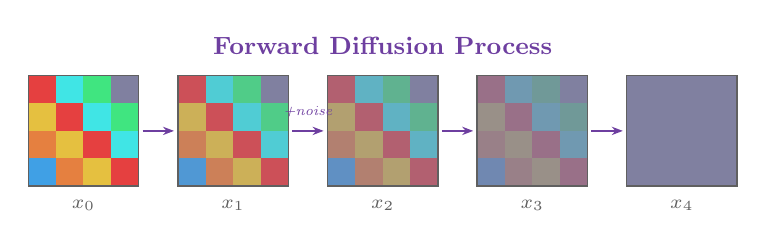
\begin{tikzpicture}

%% COPY-START =========================================================

\def\xO{0}
\def\yO{0}
\def\frameSize{1.4}        % cm per image
\def\frameGap{0.5}         % cm between images
\def\pxN{4}                % pixels per side (4x4 = 16 pixels)
\def\nFrames{5}            % number of frames (x_0 ... x_T)

% --- DRAW FRAMES ---
\foreach \f in {1,...,\nFrames} {
  \pgfmathsetmacro\fX{\xO + (\f - 1) * (\frameSize + \frameGap)}
  % noise level: 0 (clean) → 1 (pure noise) as f increases
  \pgfmathsetmacro\noiseLvl{(\f - 1) / (\nFrames - 1)}
  \pgfmathsetmacro\cellSize{\frameSize / \pxN}

  % Draw 4x4 pixels
  \foreach \i in {1,...,\pxN} {
    \foreach \j in {1,...,\pxN} {
      \pgfmathsetmacro\cx{\fX + (\j - 0.5) * \cellSize}
      \pgfmathsetmacro\cy{\yO + (\pxN - \i + 0.5) * \cellSize}
      % Pick a pixel color based on (i,j) for variety
      \pgfmathtruncatemacro\cidx{int(mod(\i * 3 + \j * 5, 8) + 1)}
      % Blend with grey based on noise level
      \pgfmathsetmacro\opVal{int(100 * (1 - \noiseLvl))}
      \fill[px\cidx!\opVal!px8]
        (\cx - \cellSize/2, \cy - \cellSize/2) rectangle
        (\cx + \cellSize/2, \cy + \cellSize/2);
    }
  }

  % Frame border
  \draw[acaGreyLine, line width=0.5pt]
    (\fX, \yO) rectangle (\fX + \frameSize, \yO + \frameSize);

  % Label (x_0, x_1, ..., x_T)
  \pgfmathtruncatemacro\labelIdx{\f - 1}
  \node[anchor=north, font=\scriptsize, color=acaGreyLine]
    at (\fX + \frameSize/2, \yO - 0.05) {$x_{\labelIdx}$};
}

% --- ARROWS BETWEEN FRAMES ---
% Note: TikZ () coords don't auto-evaluate expressions like (\arrXA + 0.05).
% Must pre-compute with \pgfmathsetmacro OR wrap with ({...}).
\foreach \f in {1,...,4} {        % nFrames - 1 arrows
  \pgfmathsetmacro\arrXA{\xO + \f * \frameSize + (\f - 1) * \frameGap}
  \pgfmathsetmacro\arrXB{\xO + \f * \frameSize + \f * \frameGap}
  \pgfmathsetmacro\arrAStart{\arrXA + 0.05}
  \pgfmathsetmacro\arrBEnd{\arrXB - 0.05}
  \pgfmathsetmacro\arrY{\yO + \frameSize/2}
  \draw[-{Stealth[length=4pt]}, line width=0.6pt, color=acaPurpleLine]
    (\arrAStart, \arrY) -- (\arrBEnd, \arrY);
  % Tiny "add noise" label above middle arrow only
  \ifnum\f=2
    \pgfmathsetmacro\labX{(\arrXA + \arrXB) / 2}
    \pgfmathsetmacro\labY{\arrY + 0.05}
    \node[anchor=south, font=\tiny\itshape, color=acaPurpleLine]
      at (\labX, \labY) {+noise};
  \fi
}

% --- TITLE ---
\pgfmathsetmacro\titleX{\xO + (\nFrames * \frameSize + (\nFrames - 1) * \frameGap) / 2}
\pgfmathsetmacro\titleY{\yO + \frameSize + 0.15}
\node[anchor=south, font=\small\bfseries, color=acaPurpleLine]
  at (\titleX, \titleY)
  {Forward Diffusion Process};

%% COPY-END ===========================================================

\end{tikzpicture}
\end{document}
